% !TEX encoding = UTF-8
% !TEX TS-program = pdflatex
% !TEX root = ../tesi.tex
% !TEX spellcheck = it-IT

%**************************************************************
\chapter{Stage}
\label{cap:stage}
%**************************************************************

%\intro{Breve introduzione al capitolo}\\

%**************************************************************
\section{Pianificazione del lavoro}

Per raggiungere gli obiettivi pianificati nel piano di stage e rispettare i requisiti minimi imposti dall'Università, io e il tutor aziendale abbiamo previsto 320 ore di lavoro, distribuite in 8 settimane da 40 ore ciascuna. Ho iniziato lo stage il 26/09/2016 e ho terminato, a causa di un giorno di festività, nel lunedì 21/11/2016, rimanendo in linea con quanto preventivato inizialmente, senza incorrere in imprevisti.

	\subsection{Definizione del piano di lavoro}
	
	Un mese prima dell'inizio dello stage ho redatto un Piano di Lavoro, definendo gli obiettivi e la pianificazione delle attività a granularità settimanale, elencando nel dettaglio i compiti da svolgere per ogni fase. Ho specificato inoltre le modalità di interazione col tutor, revisioni di avanzamento e una previsione delle competenze guadagnate dallo stagista alla fine delle attività. Le fasi identificate in tale documento sono:
	
	\begin{itemize}
		\item \textbf{Formazione teorica}: durante la prima fase del percorso formativo il tirocinante viene introdotto alle modalità di approccio alla programmazione web mediante: 
			\begin{itemize}
				\item utilizzo dell'ambiente di sviluppo Eclipse per implementazioni e \textit{debug};
				\item studio della piattaforma Java EE, integrazione di \textit{application server} e utilizzo di diverse JVM;
				\item implementazione di interfacce grafiche tramite JSP;
				\item studio di framework di uso comune come Struts, Hibernate e Maven;
				\item sviluppo delle funzionalità mediante l'utilizzo di linguaggi Java e JavaScript.
			\end{itemize}
		\item \textbf{Formazione pratica}: in questa fase lo stagista inizia a lavorare a stretto contatto con il resto del gruppo di lavoro, imparando come affrontare correttamente le attività da un punto di vista sia tecnico sia analitico. Vengono utilizzati i sistemi di versionamento per lo sviluppo di programmi di esempio, dai più semplici (solo Java) ad una completa applicazione web in tecnologia Java EE, secondo la metodologia di lavoro corretta. Questo periodo termina con l'analisi della struttura di una complessa applicazione reale.
		
		\item \textbf{Sviluppo su applicazione reale}: analisi e implementazione di modifiche relative ad attività reali dell'applicazione ELISE, progetto di stage, in affiancamento al gruppo di lavoro. Il tirocinante si impegna ad analizzare e successivamente stimare le attività che gli verranno assegnate portandole a compimento al pari di una qualsiasi delle figure del team nelle giuste tempistiche.		
	\end{itemize}
	
	\begin{figure}[H]
		\centering
	   	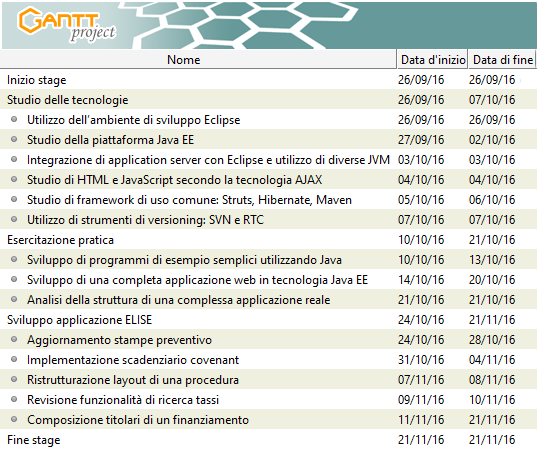
\includegraphics[width=1\textwidth]{immagini/tabella_gantt}
	   	\caption{Pianificazione delle attività di stage}
	\end{figure}
		
	Questa pianificazione dettagliata mi ha permesso di distribuire il carico di lavoro e di verificare l'allineamento tra il lavoro effettivamente svolto e il lavoro pianificato, al termine di ogni settimana.	
	
	\subsection{Livello di autonomia}
	
	Durante lo svolgimento dello stage il tutor aziendale è stato disponibile per ogni mia necessità, fornendomi consigli riguardo le tecnologie che andavo ad affrontare, specie nelle	prime fasi. Ho lavorato in un ambiente che mi consentiva di essere a stretto contatto con lui in modo da favorire l'interazione e garantire il raggiungimento degli obiettivi prefissati.\\
	
	Sono state effettuate verifiche di avanzamento sia settimanali che giornaliere, quando ritenuto necessario, con relativa revisione dei prodotti per assicurarsi del corretto punto di completamento rispetto alla pianificazione concordata in partenza.\\
	
	Una volta presa confidenza con gli ambienti e la strumentazione aziendale, ho avuto modo di agire liberamente nelle mie attività, ricevendo dal tutor solo indicazioni sulla strada da percorrere e sui vincoli da rispettare. Successivamente sono stato capace di lavorare in maniera autonoma, com'era desiderabile aspettarsi, ricevendo solo qualche saltuaria delucidazione.	
	
%**************************************************************
\section{Studio degli strumenti di sviluppo}

Con il mio arrivo in azienda è iniziata la prima fase del lavoro di stage, ovvero lo studio delle tecnologie adottate dalla divisione Servizi Finanziari per l'adempimento dei suoi scopi. L'obiettivo era quello di conferirmi una formazione teorica da consolidare in seguito con delle prove pratiche a scopo esercitativo.\\

Nelle prime settimane ho quindi studiato i linguaggi, le tecniche di progettazione e gli ambienti di sviluppo che assieme al tutor aziendale avevo pianificato di trattare nel piano di lavoro. Nelle settimane successive avrei poi messo in pratica e ottenuto padronanza di tali tecnologie secondo le metodologie aziendali, approfondendo le conoscenze su tali argomenti, in preparazione alla fase di sviluppo sull'applicazione ELISE.

	\newpage

	\subsection{Tecnologie utilizzate}

	\subsubsection{Piattaforma web}
	Java Platform Enterprise Edition, o Java EE, è un'estensione di Java SE (Standard Edition) e rappresenta una piattaforma di sviluppo software molto usata per applicazioni d'impresa.\\
	
	Java EE è sviluppato mediante il Java Community Process, ovvero un processo che permette ad una comunità di esperti industriali, organizzazioni (commerciali e \textit{open source}) e un'infinità di individui di dare il loro contributo seguendo determinati standard. Esso fornisce gli strumenti utili per la programmazione web, tra cui un ambiente \textit{runtime} e librerie utili allo sviluppo di applicazioni distribuite, scalabili, affidabili e sicure che prevedono Java come linguaggio di programmazione primario.\\
	
	\begin{figure}[H]
		\centering
	   	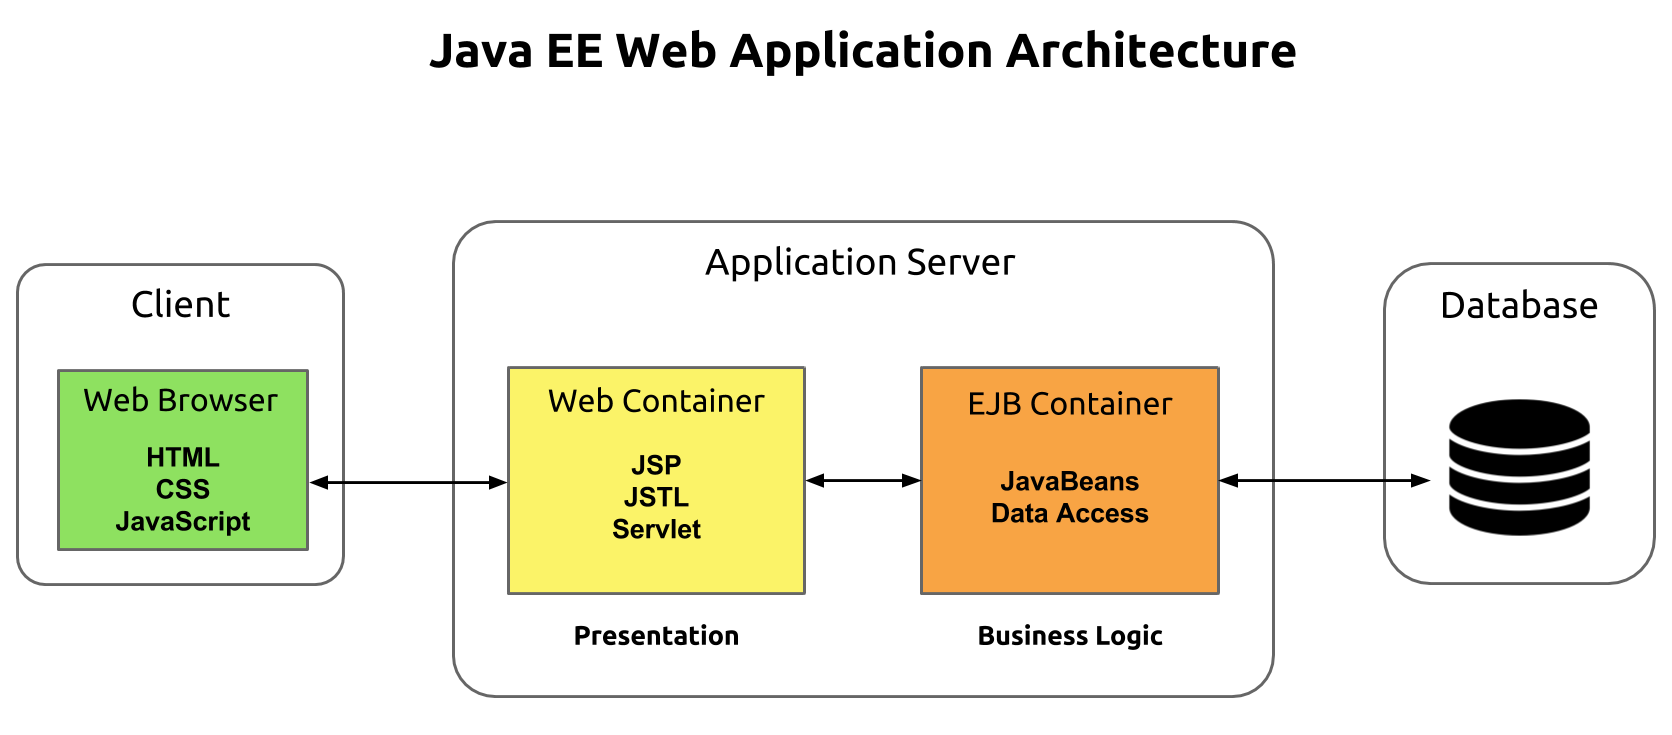
\includegraphics[width=1\textwidth]{immagini/architettura_javaEE}
	   	\caption{Architettura di un'applicazione sviluppata in Java EE}
	\end{figure}
	
	Utilizzando Java EE risulta fondamentale l'utilizzo di un \textit{application server} (o \textit{servlet}\glossario\ \textit{container}) per l'esecuzione e la distribuzione dell'applicativo nei diversi nodi della rete.
	Si tratta di un ambiente che estende le funzionalità offerte da un normale Web Server, ovvero il paradigma client-server e la comunicazione dei contenuti mediante protocolli web. Esso è strutturato nei diversi livelli architetturali (architettura multi-tier) di cui un'applicazione web ha bisogno per eseguire:
	
	\begin{itemize}
		\item \textbf{Presentation layer}: rappresenta la logica di presentazione delle pagine web dell'applicazione;
		\item \textbf{Business layer}: strato della logica funzionale dell'applicazione, utile per la generazione di contenuti dinamici;
		\item \textbf{Persistent layer}: ovvero la gestione dei dati e della loro persistenza.
	\end{itemize}
	
	Sono disponibili diversi \textit{application server} tra cui JBoss (RedHat) e WebSphere (IBM) e servlet container come Tomcat (Apache).\\
	
	La piattaforma Java EE adotta una convenzione per la configurazione mediante XML delle componenti dell'applicazione, in particolare 
	il file web.xml (contenuto in \textit{WebContent/WEB-INF/}) contiene le impostazioni principali riguardanti la gestione delle richieste inviate al server.\\
	
	\begin{figure}[H]
		\centering
	   	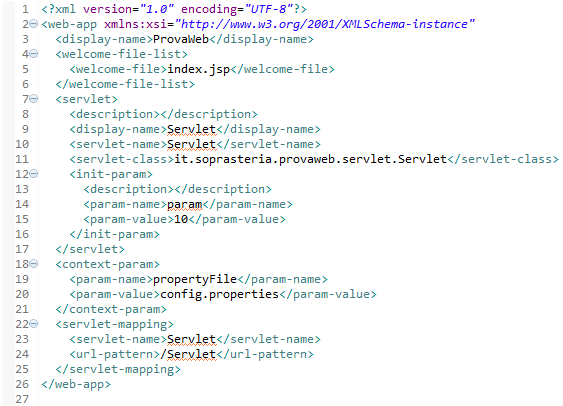
\includegraphics[width=1\textwidth]{immagini/web_xml}
	   	\caption{Un esempio di configurazione imposta tramite il file web.xml - Fonte: ambiente di sviluppo in Eclipse}
	\end{figure}
	
	Quando si compila un applicazione Java EE viene generato un JAR\glossario\ (Java Archive) di tipo EAR (Enterprise Archive) o WAR (Web Archive), questi file vengono eseguiti rispettivamente dall'\textit{application server} e dal \textit{servlet}\glossario\ \textit{container}, due framework che si occupano quindi di avviare l'applicazione. 
	
	\subsubsection{Presentazione}
	
	Per la creazione delle interfacce grafiche delle applicazioni durante lo stage, ho utilizzato gran parte delle tecnologie standard, ovvero HTML, CSS per l'aspetto e la struttura e JavaScript per il comportamento. Tali tecnologie erano già di mia conoscenza e non richiedevano troppo impegno da parte mia.\\
	
	I contenuti generati con queste tecnologie, però, sono stati inglobati in un ambito di cui io non ero ancora a conoscenza: le pagine JSP.\\
	
	JSP (Java Server Pages) è una tecnologia di programmazione web in Java EE per lo sviluppo della logica di presentazione delle applicazioni, eseguito tipicamente fornendo contenuti dinamici in formato HTML e inglobando le tecnologie citate prima. Al momento della compilazione del software, tali pagine vengono lette dal compilatore JSP e trasformate nelle apposite classi Java Servlet\glossario , ovvero una specifica estensione di Java pensata per l'utilizzo web.
	
	\begin{figure}[H]
		\centering
	   	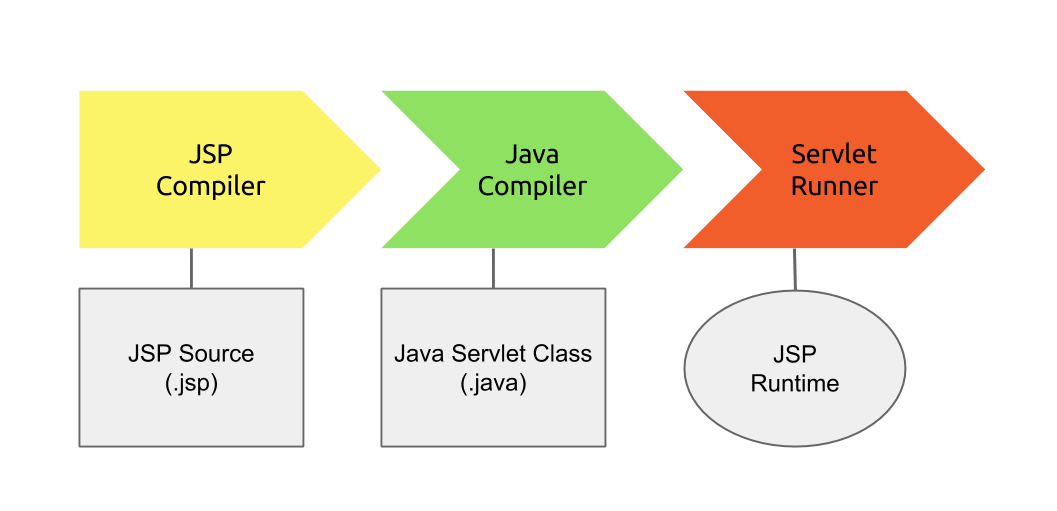
\includegraphics[width=1\textwidth]{immagini/jsp_compile}
	   	\caption{Flusso di compilazione di una JSP}
	\end{figure}
	
	\begin{figure}[H]
		\centering
	   	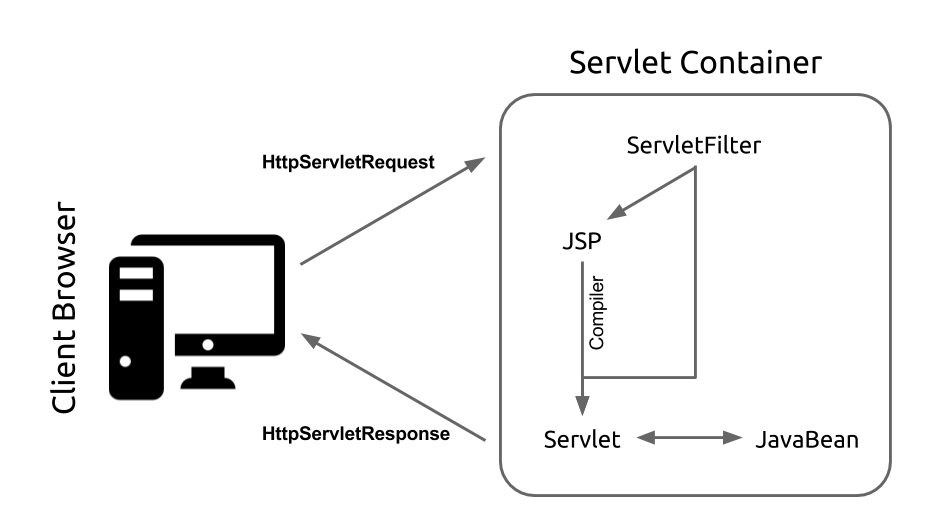
\includegraphics[width=1\textwidth]{immagini/jsp_comunications}
	   	\caption{Rappresentazione della cominicazione client-server in ambito JSP}
	\end{figure}	
	
	All'interno di una JSP viene definito l'HTML in cui viene immerso il codice Java sottoforma di \textit{scriptlet}. Il tutto viene poi compilato e come risultato viene prodotta una Java Servlet\glossario . In particolare questo tipo di classi fornisce al programmatore la possibilità di manipolare la comunicazione client-server mediante appositi oggetti. A questo punto, il codice HMTL viene stampato in pagina mediante l'oggetto \textit{HttpServletResponse}.\\
	
	Queste pagine si basano anche su un insieme di librerie di tag JSTL (Java Standard Tag Library), con cui possono essere invocate funzioni predefinite sotto forma di classi Java. In aggiunta, permette di creare librerie di nuovi tag che estendono l'insieme dei tag standard (JSP Custom Tag Library).
	
	\subsubsection{Framework}
	Durante il lavoro di stage ho sempre utilizzato il framework Struts, in particolare per lo sviluppo delle nuove funzionalità per l'applicazione ELISE dell'ultima fase.\\
	
	Si tratta di uno strumento utile alla creazione di applicazioni sviluppate secondo Java EE. Nella fase di studio delle tecnologie ho avuto modo di comprendere la sua forza, anche grazie alle mie conoscenze, acquisite durante il corso di studi. Struts infatti estende le Java Servlet\glossario , implementando il design pattern MVC\glossario\ (Model-View-Controller), definendo una solida struttura per il software che lo adotta. 
	
	\begin{figure}[H]
		\centering
	   	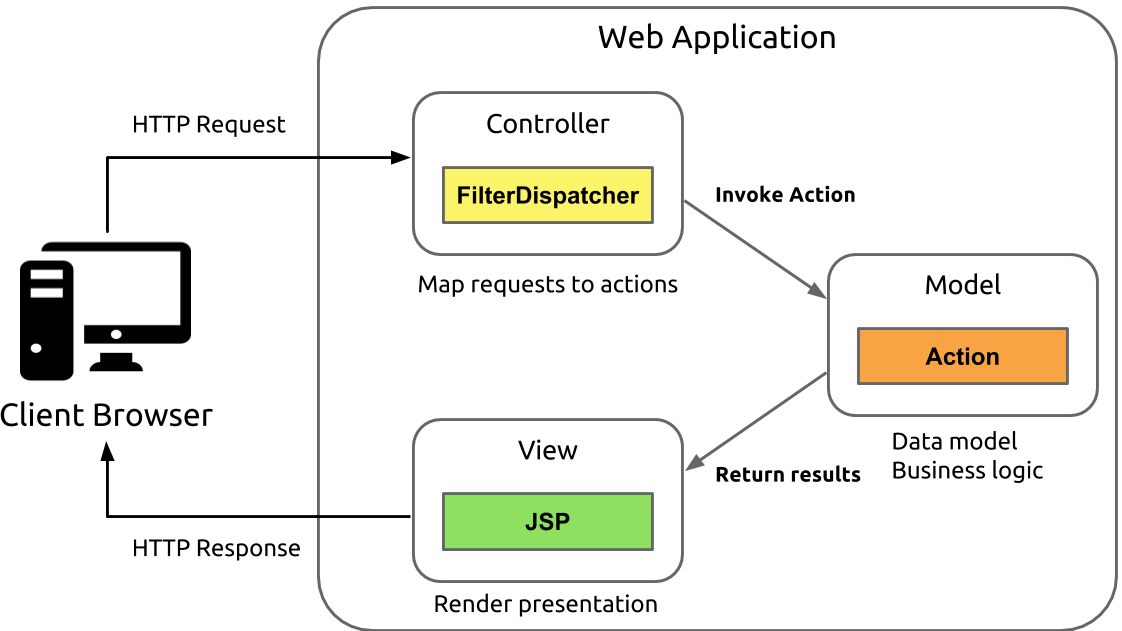
\includegraphics[width=1\textwidth]{immagini/MVC_struts}
	   	\caption{Struttura di un'applicazione sviluppata mediante il design pattern imposto da Struts}
	\end{figure}	
	
	L'utilizzo di questo framework permette lo sviluppo di applicazioni web di notevoli dimensioni, inoltre agevola la suddivisione dello sviluppo del progetto fra i vari dipendenti. I programmatori web e i vari gruppi di sviluppatori possono quindi gestire in parallelo e autonomamente la loro parte del progetto.\\
	
	Questo risulta maggiormente utile se si associano le proprie attività di sviluppo ad un sistema di versionamento, dove poter integrare le porzioni di software, ben strutturato secondo il framework.
	
	\subsubsection{Properties}	
	Data la grandezza del progetto ELISE ed il suo elevato numero di pagine, è stato adottato un meccanismo per la gestione delle \textit{label}, ovvero le scritte statiche da presentare in pagina.\\
	
	In particolare grazie alla tecnologia JNDI\glossario\ è possibile creare un vocabolario (memorizzato su file .properties) di stringhe Java, codificate mediante un nome identificativo, da richiamare nelle pagine JSP in modo da facilitare il mantenimento e la modifica di tale aspetto.\\
	
	\begin{figure}[H]
		\centering
	   	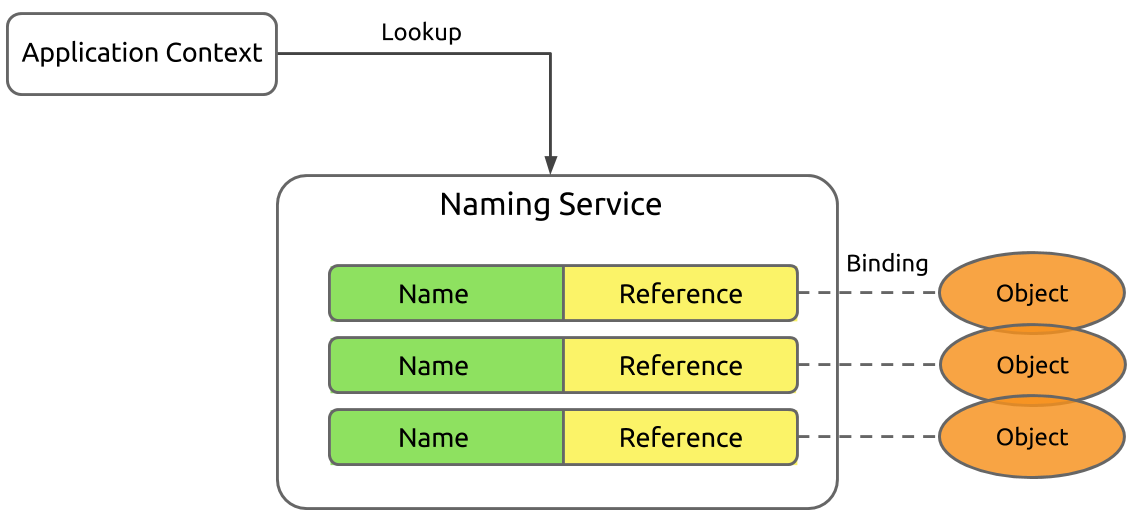
\includegraphics[width=1\textwidth]{immagini/JNDI}
	   	\caption{Sistema di vocabolario generato dall'uso di JNDI}
	\end{figure}	
	
	Ovviamente in questo modo più pagine possono riferirsi alla stessa stringa utilizzando lo stesso identificativo, nel momento in cui un label deve essere modificato basterà cambiarlo nel vocabolario e tutte le pagine che si riferiscono ad esso verranno aggiornate.
	
	\subsubsection{Logging}	
	Una tecnica molto utile che ho imparato durante dello stage è l'uso dei log, che nel percorso di studi avevo solo visto a grandi linee nel corso di Programmazione Concorrente e Distribuita.\\
	
	Tale tecnica prevede di utilizzare di un servizio, spesso una libreria esterna, per tracciare il flusso applicativo e stampare su file le informazioni rilevanti dei vari stati che il software ha incontrato durante la sua esecuzione. Nel mio caso è stato adottato Log4J, una libreria molto nota a questo scopo, utilizzata anche nel progetto ELISE.\\
	
	Essa permette di emettere delle notifiche nei vari punti del software, associandone il livello di importanza e livello generale dell'applicativo impostare il livello di debug da utilizzare durante l'esecuzione. Una volta lanciato, il programma produrrà il log contenente solo le notifiche che rispettano il livello selezionato, nascondendo quelle di minore importanza.\\
	
	\begin{figure}[H]
		\centering
	   	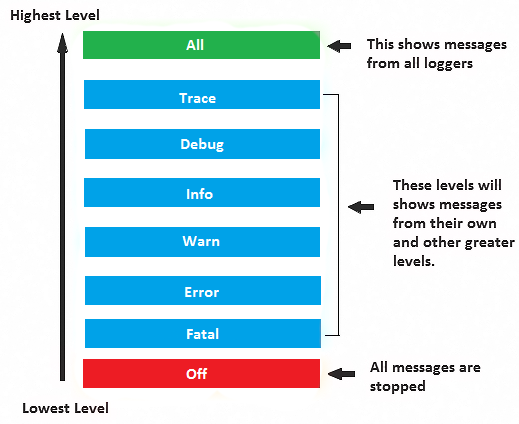
\includegraphics[width=1\textwidth]{immagini/log_levels}
	   	\caption{I diversi livelli di log selezionabili con la libreria Log4J - Fonte: tutorial online sull'uso della libreria}
	\end{figure}	
	
	In molte occasioni è stato necessario consultare i file di log per risalire ad eventuali errori oppure per comprendere meglio il comportamento dell'applicazione. Talvolta è stato scelto di modificare il livello di debug per analizzare più a fondo i messaggi prodotti dal software.
	
	\subsubsection{Stampe PDF}	
	Un'altra tecnica adotata dal progetto ELISE è la generazione dinamica di documenti PDF, da produrre nella filiale di competenza che li deve stampare per conto degli utenti allo	sportello.\\
	
	Per ottenere tutto questo sono previste delle classi Java specifiche dell'applicativo che si servono della libreria iText per l'inizializzazione di un documento ed il relativo riempimento con i giusti contenuti, sotto forma di tabelle, paragrafi, frasi, ecc. Anche questa libreria è tra le più usate per questo scopo, il che rende facile reperire guide e documentazione ufficiale su internet.
	
	\begin{figure}[H]
		\centering
	   	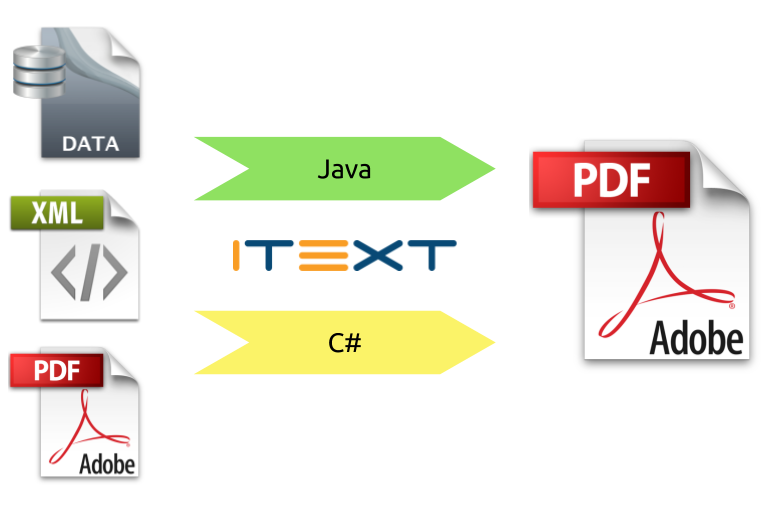
\includegraphics[width=1\textwidth]{immagini/itext}
	   	\caption{Illustrazione del processo di creazione dei documenti PDF mediante la libreria iText}
	\end{figure}
	
	\subsection{Alternative analizzate}
	
	\subsubsection{Hibernate}	
	Hibernate è un framework \textit{open source} per lo sviluppo di applicazioni Java. Fornisce un servizio di \textit{object-relational mapping} (ORM) ovvero gestisce la persistenza dei dati sul database attraverso la rappresentazione e il mantenimento su database relazionale di un sistema di oggetti Java. Come tale dunque, nell'ambito dello sviluppo di applicazioni web, si frappone tra il livello logico di business e quello di persistenza dei dati sul database.\\
	
	La funzione primaria di Hibernate quindi, è di mappare classi Java in tabelle del database e tipi di dati Java in tipi di dati SQL. Questo framework non è adottato dal team per questo progetto in quanto la persistenza dei dati mediante un sistema CICS\glossario\ non è supportata. Infatti il processo di codifica del	flusso dati per comunicare con l'ambiente \textit{host} è già ampiamente gestito mediante apposite classi Java che, con l'uso della Reflection e di mappe XML, si occupano di generare gli appositi JavaBean\glossario .
	
	\subsubsection{Spring}	
	Spring è un altro framework \textit{open source} per lo sviluppo di applicazioni su piattaforma Java. L'aspetto centrale nell'utilizzo di Spring è avere a disposizione il suo \textit{inversion of control container}, ovvero un ambiete che invita lo sviluppatore ad applicare il design pattern architetturale \textit{dependency injection}, permettendo di gestire in maniera consistente oggetti Java usando la Reflection.\\
	
	Il contenitore si occupa del ciclo di vita degli oggetti gestiti, detti beans, mediante una configurazione fornita su file XML. Oltre a questa funzionalità, il framework offre supporto ad attività di \textit{transaction management}, accesso ai dati, messaggistica e verifica. Spring non è adottato nello sviluppo di ELISE in quanto il progetto è già ampiamente strutturato secondo il framework Struts.
	
	\subsubsection{Maven}	
	Apache Maven è un framework per la gestione di un progetto software. Esso può gestire la compilazione del progetto, l'invio di segnalazioni e la documentazione basandosi sul concetto centrale di \textit{project object model} (POM), un file XML che descrive le dipendenze fra il progetto e le varie versioni di librerie necessarie.\\
	
	Maven effettua automaticamente il download di librerie Java e plug-in Maven dai vari repository definiti, scaricandoli in locale o in un repository centralizzato lato sviluppo. Questo permette di recuperare in modo uniforme i vari file JAR\glossario\ e di poter spostare il progetto indipendentemente da un ambiente all'altro avendo la sicurezza di utilizzare sempre le stesse versioni delle librerie.\\
	
	Questo framework è stato da me studiato solo a scopo formativo, in quanto l'ambito di progetto non richiedeva di usufruire delle funzionalità che esso offre. In particolare la portabilità del software trattato è garantita dall'utilizzo degli ambienti di collaudo del cliente, senza bisogno di renderlo compatibile con altre macchine.
	
	\subsubsection{SVN}	
	SVN (Subversion, Apache) è un sistema di versionamento, già descritto in sezione \ref{sistemi-versionamento}, alternativo ad RTC. È stato analizzato da parte mia a scopo formativo ed è utilizzato da parte dell'azienda per lo sviluppo altri progetti.

%**************************************************************
\section{Processo di sviluppo}

Al termine delle prime due fasi, come pianificato, il lavoro di stage aveva occupato un mese, metà del tempo a disposizione. Come ultima attività ho svolto un'analisi conoscitiva dell'applicazione ELISE, a cui avrei poi partecipato nello sviluppo. Mi preparavo quindi ad entrare nell'ultima fase, quella di implementazione delle espansioni su di un applicativo reale, per occupare il restante 50\% del lavoro.\\

	\subsection{Analisi dei requisiti}
	
	Come prima attività, per reperire il lavoro da svolgere, l'azienda esegue delle attività di consulenza e stabilisce i contratti con i clienti. Successivamente è tutto pronto, a livello burocratico, per concentrarsi sulle esigenze del cliente e raccogliere i suoi requisiti.\\
	
	Seguendo la struttura di governo aziendale, i team di analisti si confrontano con i responsabili tecnici e direttivi dell'ente che richiede il lavoro. In questa fase l'azienda si concentra molto per stabilire al meglio i requisiti del cliente, analizzando con cura i suoi bisogni e cercando di capire quali soluzioni possono soddisfarli. In questo modo garantisce che le successive attività di progettazione e codifica avvengano su una base solida, senza il rischio di dover ripetere attività successive a causa di errori a monte del progetto.\\
	
	 Questo processo avviene solitamente mediante trasferte da parte dei consulenti o, in caso di piccole attività, anche per via telefonica. Viene redatto, come output, un documento di programmazione delle macro attività da svolgere, che resta in mano ai project manager. Oltre a questo documento, gli analisti si occupano di redigere anche un'Analisi Funzionale per ognuna delle attività.\\
	 
	 Tale documento affronta i requisiti ad alto livello, enunciando le principali funzionalità ed i cambiamenti rispetto alla versione attualmente in produzione dell'applicativo. \\
	
	Le sezioni principali di questo documento sono:
	
	\begin{itemize}
		\item \textbf{Matrice dei requisiti}: enunciato discorsivo per introdurre il problema proposto;
		\item \textbf{Descrizione funzionale}: per spiegare il comportamento dell'applicativo lato web, presentando anche un'anteprima delle pagine che verranno aggiunte;
		\item \textbf{Casi oggetti di collaudo}: qui vengono indicate le componenti che saranno analizzate in fase di testing per verificarne il corretto comportamento;
		\item \textbf{Dettaglio tecnico}: qui vengono segnalate solo alcune particolarità e vengono enunciate le componenti software che saranno modificate o aggiunte.	
	\end{itemize}
	
	Questo documento di analisi risulta di primaria importanza per la programmazione delle interfacce. Sotto il punto di vista di un programmatore web infatti, è necessario comprendere come le pagine andranno strutturate e quale comportamento dovrà adottare l'applicazione in risposta alle interazioni con l'utente o l'ambiente \textit{host}.\\
	
	Nel mio lavoro di stage ho dovuto svolgere diverse attività e per ciascuna di esse avevo a disposizione tale documento, da poter consultare in ogni momento oltre ad un approfondito studio iniziale, prima di sviluppare alcuna componente.\\
	
	Per le attività a cui sono stato assegnato, mi sono occupato di analizzare il problema in questione e di catalogare i requisiti che mi venivano forniti dagli analisti, oltre a raccoglierne di nuovi. Ho attribuito ai requisiti la seguente forma:
	
	\begin{center}
		\texttt{Importanza Tipologia - Identificativo \hspace{1cm} Titolo}
	\end{center}
	
	Dove:
	
	\begin{itemize}
		\item \textbf{Importanza}: denota il peso del requisito di riferimento e ne stabilisce una priorità. Assume i valori:
		\begin{itemize}
			\item \textbf{O}: Obbligatorio, il requisito deve essere soddisfatto per considerare il progetto completo;
			\item \textbf{D}: Desiderabile, se il requisito viene implementato porta valore aggiunto al progetto ma non è strettamente necessario. 
		\end{itemize}
		
		\item \textbf{Tipologia}: indica la natura del requisito e assume i seguenti valori:
		\begin{itemize}
			\item \textbf{F}: Funzionale, rappresenta una funzionalità che il prodotto finale dovrà fornire, che sia essa espressa in forma generale a livello di sistema o espressa nel dettaglio delle componenti;
			\item \textbf{V}: Di vincolo, specifica un vincolo che il software deve rispettare;
			\item \textbf{P}: Prestazionale, si tratta di una caratteristica di performance che il prodotto deve soddisfare;
			\item \textbf{T}: Tecnico, ovvero un requisito implementativo che l'applicazione dovrà possedere per garantire determinate funzioni.
		\end{itemize}
		
		\item \textbf{Identificativo}: un numero, generato per incremento, che identifica il requisito in modo univoco se considerato assieme alla codifica della sua importanza e tipologia;
		
		\item \textbf{Titolo}: una breve descrizione del requisito e dei suoi riferimenti.
	\end{itemize}
	
%	Di seguito ho raccolto e catalogato in una tabella i requisiti relativi alle attività del mio lavoro di stage.\\
	
%	\begin{table}[H]
%		\def\arraystretch{1.2}
%		\begin{tabular}{ | p{2cm}  p{10cm} | }
%		
%		\rowcolor{Gray}
%		\hline \textbf{Codice} & \textbf{Titolo} \\ \hline
%		
%		%Stampe preventivo:
%			OF-01 & Fornire la stampa della nuova documentazione di preventivo \\ \hline
%			DF-02 & Generare un'apposita gerarchia di classi per la documentazione di preventivo \\ \hline		
%		%Scadenziario covenant:
%			OF-03 & Fonrire la possibilità di visualizzare le scadenze covenant \\ \hline
%			DF-04 & Fornire un calendario intuitivo a livello grafico per le scadenze covenant \\ \hline
%			OF-05 & Possibilità di visualizzare il dettaglio delle scadenze covenant per data \\ \hline		
%		%Composizione titolari:
%			OF-06 & Visualizzare i titolari di un finanziamento \\ \hline
%			OF-07 & Consentire il censimento delle categorie fiscali dei titolari \\ \hline
%			OF-08 & Collegare la pagina dei titolari alla procedura di erogazione \\ \hline
%			DF-09 & Possibilità di stampare una bozza PDF della documentazione titolari \\ \hline		
%		%Ricerca tassi:
%			OP-10 & Generare una maschera di filtro che agisca sulle date di validità dei tassi \\ \hline		
%		%Layout iframe:
%			OF-11 & Permettere lo spostamento della finestra per il web service esterno \\ \hline
%			OF-12 & Permettere il ridimensionamento della finestra per il web service esterno \\ \hline
%			OV-13 & Realizzare gli effetti per l'iframe usando il linguaggio JavaScript \\ \hline
%			DP-14 & Rendere fluidi e gradevoli i movimenti dell'iframe per il web service \\ \hline		
%		%Generale:
%			OV-15 & Seguire lo standard dettato dall'applicazione in termini di oggetti
%				grafici e creazione di funzionalità somiglianti a quelle presenti \\ \hline
%			OV-16 & Uso di itext per la generazione dei PDF di stampa \\ \hline
%			OV-17 & Seguire il template fornito dal cliente per i documenti di stampa \\ \hline	
%		
%		\end{tabular}
%		\vspace{1mm}
%		\caption{Tabella dei requisiti delle attività implementative di stage}
%	\end{table}

	In totale, per i miei ambiti ho raccolto 66 requisiti. Ho compreso le funzionalità richieste dal cliente e quelle che l'applicativo doveva implementare, analizzando le prime nel dettaglio per ricavare le seconde. Per fare ciò mi sono servito sia dei documenti di Analisi Funzionale, sia dell'esperienza del tutor e degli altri colleghi del team. Al termine delle fasi di analisi avevo i requisiti necessari per pilotare le successive attività di progettazione e sviluppo.\\
	
	Nel seguente grafico viene mostrata la suddivisione dei requisiti secondo la loro importanza.
	
	\begin{figure}[H]
		\centering
	   	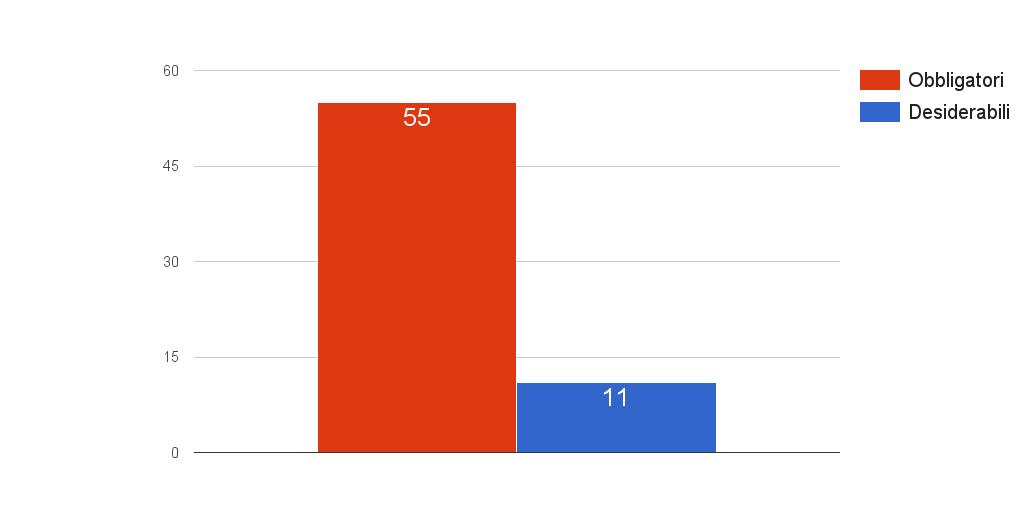
\includegraphics[width=1\textwidth]{immagini/suddivisione_requisiti2}
	   	\caption{Suddivisione dei requisiti in base alla tipologia}
	\end{figure}
	
	Nel seguente grafico mostro invece la suddivisione dei requisiti secondo la loro tipologia.
	
	\begin{figure}[H]
		\centering
	   	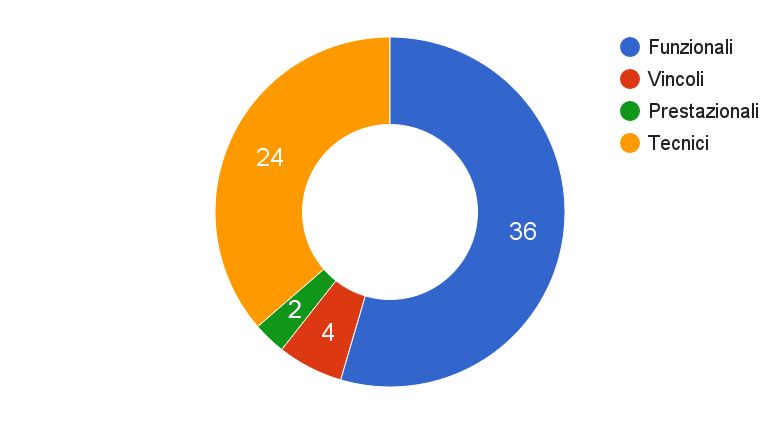
\includegraphics[width=1\textwidth]{immagini/suddivisione_requisiti}
	   	\caption{Suddivisione dei requisiti in base alla tipologia}
	\end{figure}

	\subsection{Progettazione}
	
	Le scelte architetturali sono già state prese in passato alla nascita dell'applicativo e sono radicate in tutto il software. A differenza di queste, le scelte progettuali per le singole funzionalità, che si vanno ad aggiungere col passare del tempo durante la manutenzione e l'evoluzione del software, vengono stabilite ad ogni incremento del ciclo di sviluppo. \\
	
	Terminata la fase di analisi dei requisiti, i team di competenza dell'ambiente di gestione dei dati dell'applicazione si occupano di progettare i programmi lato \textit{host}. Questa attività influenza in modo decisivo anche il modo in cui verranno poi sviluppate le interfacce web per tali programmi.\\
	
	Come output di questa fase viene prodotto quindi il documento di Specifica Tecnica. Questo secondo documento affronta nel dettaglio gli aspetti tecnici trattando principalmente i programmi COBOL\glossario , dai quali poi anche i programmatori web possono individuare i parametri da utilizzare nelle richieste via rete per recuperare i dati. In questo modo lo sviluppo delle pagine web del software viene allineato con le implementazioni fatte su \textit{host}, permettendo una progettazione corretta anche dal punto di vista dei programmatori \textit{front-end}.\\
	
	\subsubsection{Progettazione architetturale}	
	
	Lo studio della struttura di ELISE mi ha permesso di conoscere i suoi funzionamenti, comprendendo quali scelte fossero adeguate o meno in tale sistema. L'applicazione, come menzionato, si basa sul framework Struts per la definizione delle proprie fondamenta. Il vantaggio più significativo portato da tale scelta è rappresentato dalla struttura che ne deriva. \\
	
	In particolare, Struts gestisce il flusso delle richieste in entrata all'applicazione e le identifica in \textit{action} da svolgere. Queste azioni vengono definite in un apposito file XML del framework, in cui si associa una classe Java ad un URL, in modo da collegare le interazioni con l'utente nelle pagine web con la logica di business dell'applicazione. Ogni azione ha poi una pagina JSP che rappresenta il risultato delle operazioni a basso livello, Struts si occupa di eseguirne il \textit{render} una volta ottenuti i dati di cui essa ha bisogno. Spesso tali dati sono incapsulati in JavaBeans\glossario .\\
	
	Tutto ciò non sarebbe possibile se la struttura imposta dal framework non seguisse una logica ben precisa. Il software infatti implementa in questo modo un \textit{design pattern} architetturale molto usato a livello strutturale: MVC\glossario . Per l'applicazione ELISE questo pattern è implementato secondo il modello web, ovvero a partire da una pagina JSP si richiama la logica di business (sottoforma di Enterprise JavaBeans) attraverso il server (rappresentato da classi Servlet). 
	
	\begin{figure}[H]
		\centering
	   	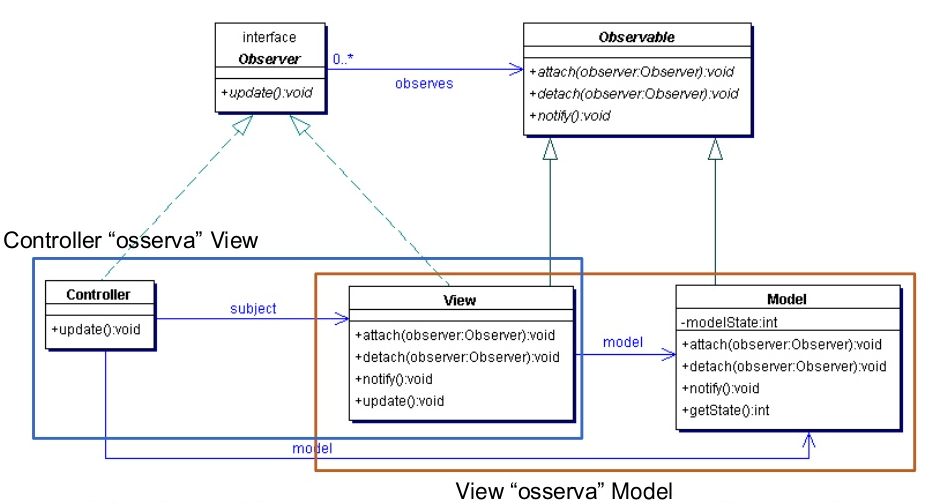
\includegraphics[width=1\textwidth]{immagini/diagramma_MVC}
	   	\caption{Diagramma delle classi per l'implementazione del \textit{design pattern} architetturale MVC - Fonte: slides del corso di Ingegneria del Software mod. B}
	\end{figure}
	
	In questo modo possono essere realizzate più viste grafiche che rimandano alla stessa componente Java, definendo le apposite parti che si occupano del controllo delle richieste e stabilendo i collegamenti nel file \textit{struts-config.xml}.
	
	\begin{figure}[H]
		\centering
	   	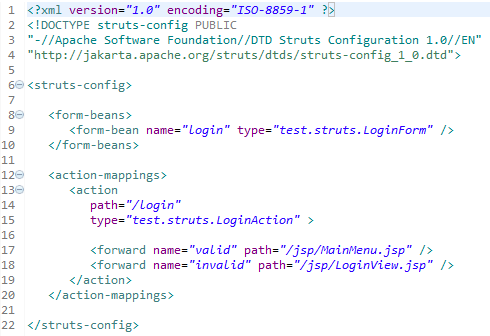
\includegraphics[width=1\textwidth]{immagini/struts_config}
	   	\caption{Esempio di configurazione delle componenti di Struts mediante file XML}
	\end{figure}	
	
	\subsubsection{Progettazione di dettaglio}
	
	Per le singole attività di manutenzione ed espansione di ELISE, la progettazione dell'applicativo avviene in base ai requisiti e agli scopi di tali modifiche. Le fasi di progettazione di dettaglio si susseguono infatti ad ogni incremento applicato sul software, allo scopo di definire in modo corretto le componenti utili al soddisfacimento dei requisiti. \\
	
	Io sono stato l'unico responsabile nel definire la struttura delle parti che componevano le mie attività. Il tutor mi ha insegnato precedentemente come agire e successivamente mi ha lasciato produrre in autonomia, revisionando il mio lavoro solo per eventuali accertamenti, ma è comunque rimasto sempre a mia disposizione.\\
	
	Per le mie attività ho quindi cercato di analizzare il problema e ideare delle soluzioni adatte all'applicazione di progetto. In particolare, come descritto, avevo già a disposizione una solida struttura e molte librerie utili. Si trattava di muovere i primi passi in quel sistema e progettare delle soluzioni che riutilizzassero quante più funzionalità già presenti. In tale ottica anche le mie soluzioni prodotte, se risultavano completamente nuove, andavano pensate per essere riutilizzate in futuro.\\
	
	Ho cercato di soddisfare i requisiti del cliente al meglio, senza fretta nel produrre subito una codifica delle soluzioni, ma pensando bene alla loro organizzazione. In questo senso mi sono impegnato a organizzare il codice in classi che rispettassero una solida gerarchia e fossero estendibili, per garantirne un'utilità futura. Ad esempio, per la gestione delle stampe dei preventivi e la documentazione della composizione dei titolari di un finanziamento, ho realizzato tale struttura per definire le varie tipologie di stampa. In tal modo ho raggruppato le parti in comune nelle classi poste in alto nella gerarchia.
	
	\begin{figure}[H]
		\centering
	   	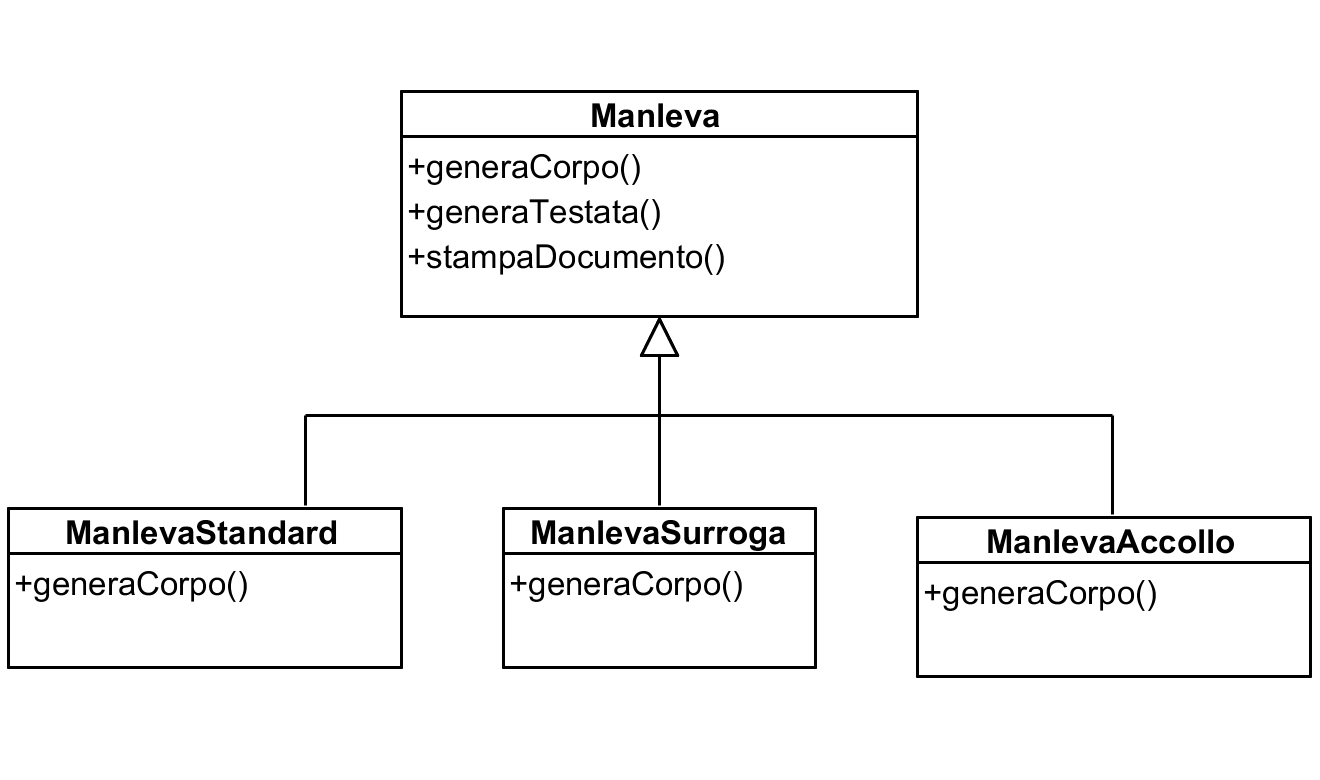
\includegraphics[width=1\textwidth]{immagini/diagramma_stampe}
	   	\caption{Diagramma delle classi semplificato della gerarchia per le stampe}
	\end{figure}
	
	Un'altra tecnica che ho avuto modo di studiare e applicare in maniera approfondita è la Reflection\glossario . L'ho usata principalmente per rendere noto al sistema software quali parti delle mie componenti dover recuperare per svolgere determinate funzioni. Nel dettaglio ho modificato e creato dei nuovi file di configurazione XML, in cui ho definito i parametri e i nomi dei campi dei JavaBeans\glossario\ da utilizzare nella comunicazione con l'ambiente \textit{host} e nelle pagine dell'applicazione.\\
	
	Per quanto riguarda la tecnologia JSP, che racchiude diversi linguaggi in sé, è stato complicato definire uno stile generale per la creazione delle interfacce.\\
	
	A tale scopo ho cercato di separare i concetti e le utilità comprese in ogni pagina, progettando piuttosto delle classi Java esterne o diverse componenti JSP  da includere poi in un file principale. Ho creato quindi un'alta coesione delle componenti, identificando il più possibile il loro scopo e suddividendole in modo da non attribuire troppe responsabilità ad una singola parte. In questo modo andavo ad aumentare il livello di accoppiamento tra di esse, ma non risultava mai eccessivo da rappresentare uno svantaggio, in quanto il prodotto di grandi dimensioni diveniva così più comprensibile e strutturato, dando modo di riutilizzare le sue componenti.\\
	
	Come già reso noto, durante il corso dello stage ho avuto modo di applicare alcuni \textit{design pattern} studiati durante i miei studi all'Università. Un secondo pattern che desidero citare è il \textit{decorator pattern}, molto usato nella progettazione delle componenti dell'applicativo. Grazie a questo principio ho implementato delle soluzioni che aggiungevano delle funzionalità o dei contenuti a delle porzioni generiche del software.
	
	\begin{figure}[H]
		\centering
	   	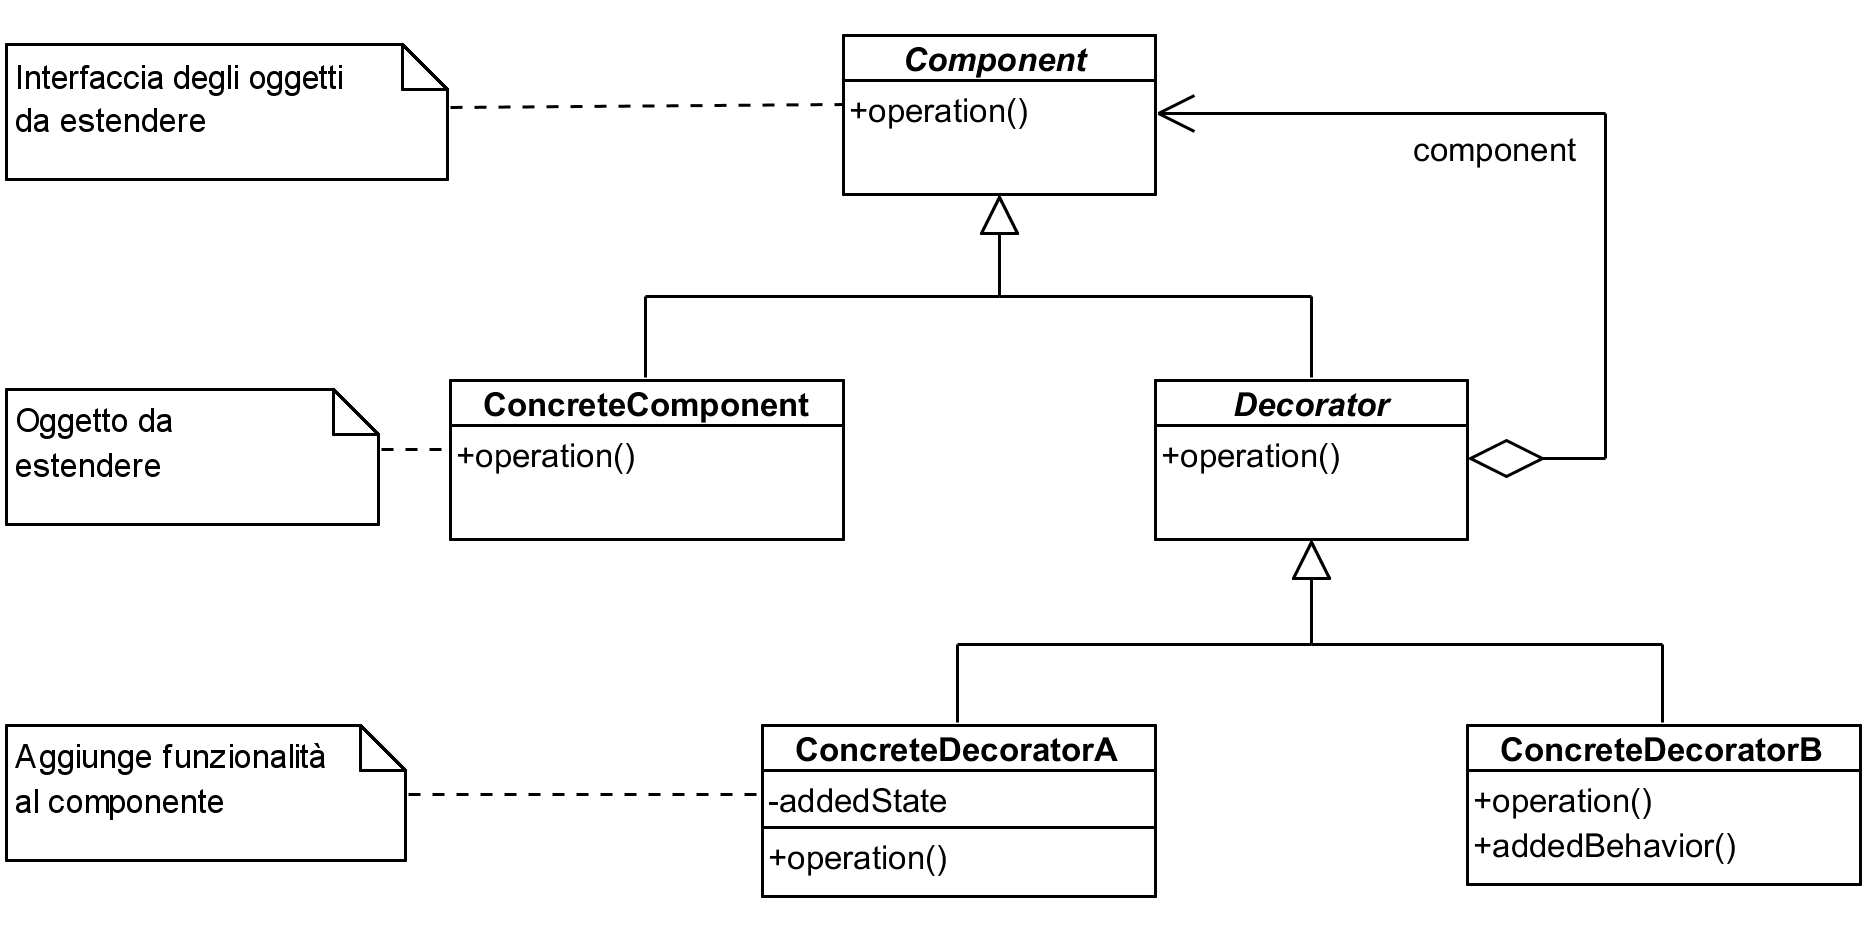
\includegraphics[width=1\textwidth]{immagini/decorator_pattern}
	   	\caption{Diagramma delle classi del \textit{decorator pattern}}
	\end{figure}
	
	\subsection{Codifica}
	
	Una volta pianificate le azioni e progettate le componenti, per ogni attività, mi sono occupato di realizzare le soluzioni.	Dal punto di vista implementativo, avere alla base del proprio lavoro un framework che si occupa di strutturare le parti del sistema e categorizzarle secondo i loro scopi, è certamente un vantaggio.\\
	
	Le fasi di sviluppo sono state quelle che più mi hanno conferito padronanza degli strumenti e delle metodologie che dovevo imparare.\\
	
	Con l'aiuto del tutor facevo chiarezza sulle implementazioni da realizzare e sulle tecniche da impiegare, guadagnando poco alla volta autonomia e responsabilità delle mie azioni. \\	
	
	Ho creato diverse pagine JSP nel corso dello stage e ho notato che tale tecnologia può causare numerose ambiguità per uno sviluppatore esterno. Organizzando il codice in modo comprensibile ho definito una struttura e raggruppato le porzioni di codice di ogni tipologia di linguaggio.	Inizialmente definivo in una \textit{scriptlet} le porzioni di codice Java utile a recuperare le componenti di business, solitamente i JavaBeans\glossario . 
	
	\begin{figure}[H]
		\centering
	   	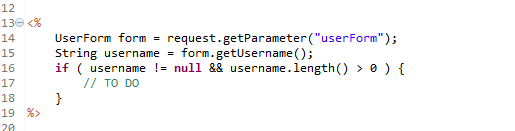
\includegraphics[width=1\textwidth]{immagini/codice_scriptlet}
	   	\caption{Esempio di codice Java incluso in una pagina JSP mediante \textit{scriptlet}}
	\end{figure}
	
	In seguito solitamente ho dato inizio alla struttura della pagina mediante i \textit{tag} personalizzati dell'applicazione, utilizzando quindi il suo \textit{template} per mantenere coerenza grafica e strutturale.\\
	
	Mi sono servito quindi dei tag standard di JSTL e ho sviluppato soluzioni con alcuni che invece sono realizzati da altri sviluppatori, come il \textit{display tag}, per la generazione di tabelle. In particolare questo tag implementa il \textit{decorator pattern}, ovvero sfrutta una classe Java appositamente realizzata per riempire la tabella con i relativi contenuti.
	
	\begin{figure}[H]
		\centering
	   	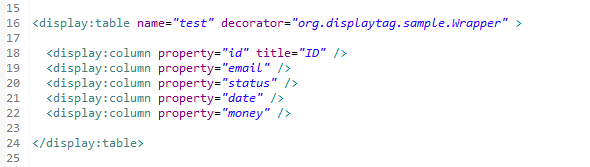
\includegraphics[width=1\textwidth]{immagini/display_tag}
	   	\caption{Esempio di codice JSP per la creazione di una tabella implementando il \textit{decorator pattern}}
	\end{figure}
	
	In seguito ho applicato le mie conoscenze di programmazione web, con i linguaggi HTML e CSS per completare la presentazione delle pagine.\\
	
	In tutte le interfacce che ho sviluppato, vi era il bisogno di definire anche un aspetto comportamentale dell'applicazione a livello client. In coda ai sorgenti delle pagine, infatti, ho inserito porzioni di codice JavaScript, utile a realizzare effetti grafici e richiamare determinate funzioni o procedure già presenti nel software.\\
	
	In tale contesto ho avuto modo di applicare la tecnica AJAX\glossario\ per recuperare determinate informazioni che risiedono nel server, senza imporre un ricaricamento della pagina. 
	
	\begin{figure}[H]
		\centering
	   	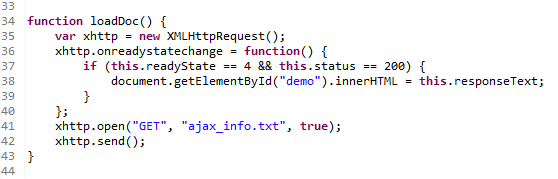
\includegraphics[width=1\textwidth]{immagini/codice_AJAX}
	   	\caption{Esempio di codice JavaScript per implementare la tecnica AJAX}
	\end{figure}

%**************************************************************
\section{Verifica e validazione}

Durante tutta la fase di implementazione delle funzionalità ho svolto anche attività di verifica e validazione. Durante la codifica ho compiuto tali attività mediante delle prove in locale, prima dei rilasci invece, attraverso un piccolo collaudo. Questo per verificare che tutti i requisiti fossero soddisfatti e che l'andamento dello sviluppo procedesse nella giusta direzione, al fine di portare in ambiente di integrazione delle soluzioni più corrette possibile ed evitare eventuali iterazioni nel ciclo di sviluppo.\\

	Io e il tutor abbiamo dato priorità a verifiche effettuate su casi di utilizzo reali dell'applicazione analizzando il funzionamento nei vari casi d'uso previsti per ogni attività, testandola quindi manualmente piuttosto che in automatico.\\
	
	Per il progetto ELISE infatti non era prevista la stesura a priori di test automatici da effettuare una volta prodotto il codice necessario, in quanto ogni attività di evoluzione, programmata per il software, si presenta ad un alto livello di granularità, garantendo una ristretta copertura di casi d'uso, facilitando quindi le attività di test.

	\subsection{Analisi statica}
	Lo strumento più usato per la verifica risulta essere l'ambiente di sviluppo Eclipse. Esso mette a disposizione dello sviluppatore un sistema di analisi statica che permette la visualizzazione di \textit{error} e \textit{warning} causati da problemi nel codice o utilizzi poco adatti del linguaggio.\\
	
	Per ogni codice sorgente che andavo ad estendere o creare, avevo la responsabilità di rimuovere tutti gli errori e limitare i \textit{warning} alle sole segnalazioni dovute all'utilizzo di versioni di JVM differenti. In tal modo si garantiva che il software non producesse malfunzionamenti dovuti ad uno scorretto uso della piattaforma Java EE.\\
	
	\begin{figure}[H]
		\centering
	   	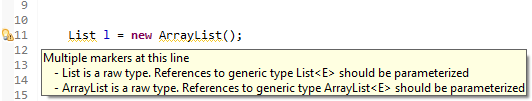
\includegraphics[width=1\textwidth]{immagini/warning_eclipse}
	   	\caption{Interfaccia di Eclipse per la segnalazione di \textit{warning}}
	\end{figure}
	
	\vspace{5mm}
	
	\begin{figure}[H]
		\centering
	   	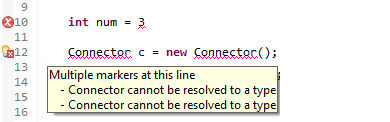
\includegraphics[width=0.8\textwidth]{immagini/error_eclipse}
	   	\caption{Interfaccia di Eclipse per la segnalazione degli \textit{error}}
	\end{figure}
	
		\vspace{5mm}	
	
	Nelle fasi di sviluppo, utilizzando Eclipse, ho inoltre avuto modo di usufruire delle sue funzionalità di \textit{debug} per il controllo di errori a tempo di esecuzione dell'applicazione. Questo mi ha permesso di scoprire errori comportamentali nel codice ma anche di comprendere i flussi intrapresi dal software durante il suo utilizzo.\\
	
	Oltre a questo strumento ho utilizzato molto i file di log generati dalla stessa applicazione, per gli stessi scopi.
	
	\subsection{Analisi dinamica}
	Nell'ultima fase di stage poi, ho svolto col supporto del tutor le attività di validazione, composte dai test di sistema e dal collaudo.
	
	\subsubsection{Test di sistema}
	Per verificare le funzionalità che doveva includere il nuovo prodotto ho effettuato i test di sistema, ovvero una serie di prove al fine di verificare la copertura dei requisiti definiti con le attività di analisi. Questi sono stati svolti in ambiente di collaudo, dove l'integrazione delle componenti dell'applicazione risulta già testata e bisogna testare l'aspetto funzionale, verificando che il prodotto presenti le funzionalità stabilite e che queste non producano errori in fase di esecuzione.\\
	
	Dopo aver compilato il codice e installato il prodotto, quindi, abbiamo testato le funzionalità da me trattate, una a una. Per prima cosa abbiamo stabilito degli scenari di prova per mappare i requisiti e abbiamo stabilito pre-condizioni e post-condizioni. Per ogni attività quindi sono state verificate le post-condizioni, accertando la copertura e il soddisfacimento dei requisiti assegnati ai vari scenari di prova.
	
	\subsubsection{Collaudo}
	Una volta effettuati i test, alcuni consulenti sono entrati in contatto con	il cliente e si sono occupati della validazione dei requisiti funzionali.\\
	
	Per tale attività vengono replicati i test di sistema, nello stesso ambiente di collaudo, per dimostrare ai clienti l'effettivo funzionamento delle \textit{feature} richieste, mostrando loro che i requisiti sono stati soddisfatti.
	
%**************************************************************
\section{Rilascio delle funzionalità}

Nell'ultima settimana di stage, il tutor ha ritenuto corretto che trattassimo anche il rilascio delle nuove \textit{feature} da me sviluppate. Col suo supporto quindi ho utilizzato il sistema di versionamento RTC, mediante Eclipse, per concludere le attività ed associarle alle apposite release unit. Così facendo ho reso disponibili le nuove funzionalità a tutto il team di sviluppo in ambiente di integrazione e, dopo una compilazione, il nuovo software risultava aggiornato.

	\begin{figure}[H]
		\centering
	   	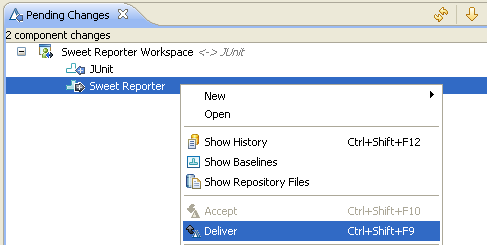
\includegraphics[width=1\textwidth]{immagini/deliver_RTC}
	   	\caption{Interfaccia per eseguire il rilascio delle attività mediante Eclipse e il sistema di versionamento RTC - Fonte: il sito internet di IBM}
	\end{figure}
	
	\begin{figure}[H]
		\centering
	   	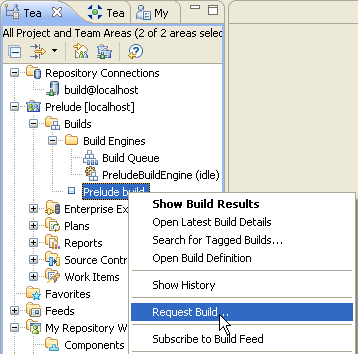
\includegraphics[width=0.6\textwidth]{immagini/build_RTC}
	   	\caption{Interfaccia per eseguire la compilazione del software in un determinato ambiente mediante Eclipse e il sistema di versionamento RTC - Fonte: il sito di RTC jazz.net}
	\end{figure}

Dopo le attività di test ho potuto effettuare i rilasci anche in ambiente di collaudo, dove ho svolto la validazione. Successivamente il cliente ha controllato il lavoro svolto, installando poi la nuova versione di ELISE nei server di produzione, per l'utilizzo vero e proprio nelle diverse filiali del gruppo del Banco Popolare.
